\chapter{Design \& Implementation}

After thoroughly researching both how fingerprinting works and how best to mitigate it, the design of the main application began.
The application that was designed and implemented is a browser add-on using the WebExtension API\@.
This is a browser add-on system that is cross-platform, compatible with Firefox, Chrome and Opera, though only Firefox was targeted due to scope and the limited timeframe available for the project.
WebExtensions have two primary types of script, one is a background script which runs across all tabs, the second is a content scrip, which is run in each tab individually.
I decided to use a combination of Firefox settings and preferences and the add-on itself to mitigate fingerprinting, as some of the settings themselves were vital to disabling fingerprinting.
The project originally aimed to do several things, outlined below.

\subsection{Alter Passive Properties}

This first feature of the application was to spoof passively transmitted properties in HTTP requests, such as User Agent.
After studying the WebExtension API, I found the \texttt{webRequest} object \citep{webRequest}.
This can have an \texttt{eventListener} attached to it to wait for a certain event to trigger, and once this event triggers, the add-on can execute code before the browser continues with the request.
Included in these events is the \texttt{onBeforeSendHeaders} event, which is what I originally used.
The full flow of a HTTP request in the browser is displayed in Figure~\ref{fig:webRequest-flow}.

\begin{figure}[h]
\caption{Showing the event flow for a HTTP request}
\fbox{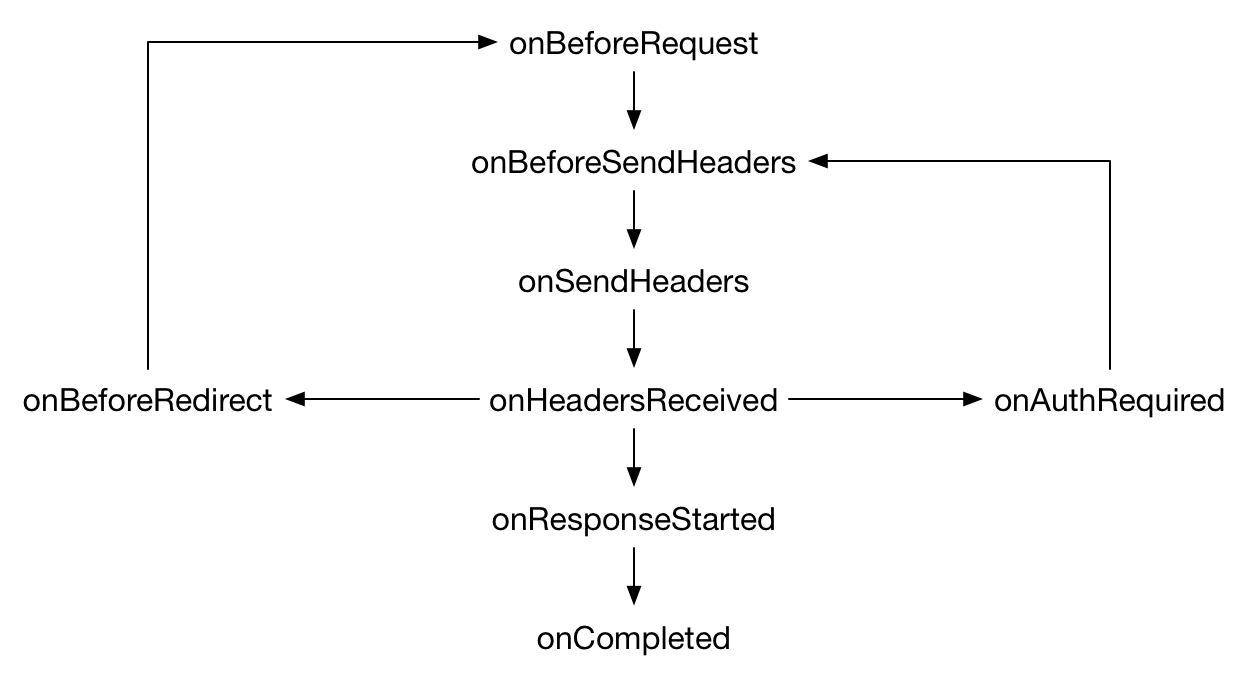
\includegraphics[scale=0.22]{webRequest-flow}}
\centering
\label{fig:webRequest-flow}
\end{figure}

The add-on in this case acts as a proxy between the browser and the website, changing the traffic before passing it on.
Listing~\ref{lst:user-agent} shows the developed background script that changes the User Agent.
Using this same method, I was able to change other headers, such as editing the date header to have a different timezone than the actual timezone of the computer or changing the HTTP\_ACCEPT headers.

\begin{lstlisting}[caption={The callback used to change the User Agent header}, label={lst:user-agent}]
var ua = "Mozilla/5.0 (Windows NT 10.0; Win64; x64) AppleWebKit/537.36 (KHTML, like Gecko) Chrome/55.0.2883.87 Safari/537.36";

function headerCallback(requestDetails) {
    for (var header of requestDetails.requestHeaders) {
        if (header.name.toLowerCase() === "user-agent") {
                        header.value = ua;
                                
        }
            
    }
        return {requestHeaders: requestDetails.requestHeaders};

}

browser.webRequest.onBeforeSendHeaders.addListener(headerCallback, {urls: ["<all_urls>"]}, ["requestHeaders", "blocking"]);
\end{lstlisting}

After doing more research, I came to realise that spoofing the User Agent for a more common user agent is only going to work against the computer against anything more than the simplest of fingerprinters.
This is because of the different functionality of different browsers can be queried and by process of elimination, the browser and version quickly identified.
By spoofing the value, it makes it more obvious to a complex fingerprinter what the user's identity is, as so few browsers spoof this information.
For this reason, the final iteration of the add-on does not alter the User Agent header.
In addition to this, the timezone header is not altered because of problems with usability for sites that depend on accurate timing information.

\subsection{Flash Prevention}
\subsection{Prevent Canvas and Audio Fingerprinting}
\subsection{Font Fingerprinting}

